\section{Design and Implementation}
\label{sec:implementation}

At the core of the \emph{GPU First} methodology is a novel compilation technique that automatically generates a GPU executable from a CPU application with (almost) arbitrary library calls, e.g., to a system or third-party library.
The most complex component of this scheme is the automatic generation of RPCs to transparently execute library functions on the host since they are not available on the GPU.
During compile time, external function calls are replaced by RPC code to perform the call remotely.
When this happens, the call arguments are automatically transferred to the host and, in case of pointers, the underlying memory is usually migrated as well.
While not infallible, our proof-of-concept scheme automatically handles the most common cases.
Limitations are discussed in more detail in \Cref{sec:limitations}.
By minimizing, often even eliminating, the manual work required to run applications on the GPU, our approach aims to facilitate the adoption of GPU acceleration and help non-experts leverage the potential of modern hardware.

\subsection{GPU Code Generation and Loading}

In contrast to classical offloading we directly target the GPU with the entire application code.
For this task we utilize an extended version of the direct GPU compilation framework by \citet{DBLP:conf/llvmhpc/TianHPCD22}.
In a nutshell, the application code is transparently enclosed in a \lstinline{#pragma omp begin/end declare target device_type(nohost)}\\ scope to utilize existing OpenMP offloading support in LLVM/ Clang to generate GPU code.
In the final executable, the application \lstinline{main} function is invoked via the OpenMP offload mechanism after command line arguments have been mapped to the device and the host RPC server has been set up.
For more information on the code generation and loading we refer to the original paper~\cite{DBLP:conf/llvmhpc/TianHPCD22}.

\subsection{Generating Remote Procedural Calls}
\label{sec:rpc-and-memory}

To identify and efficiently replace library calls in the application by RPCs we provide a dedicated link time optimization (LTO) pass.
The benefit over per translation unit reasoning is the complete world view which includes all the functions defined by the application as well as the call sites and contexts in which library functions, or simply non-defined functions, are called.
It is important to note that compared to existing LLVM-IR passes our RPC generation emits host code while the device code is analyzed and transformed.

\begin{figure}[p]
\lstset{ numbers = right,
         numbersep = 5pt, 
         numberstyle = {\color{gray}},
         stepnumber = 4,
         %numberfirstline=true,
        basicstyle=\footnotesize\lst@ifdisplaystyle\footnotesize\linespread{0.94}\fi\ttfamily,
        }
         
\ContinueLineNumber

\begin{minipage}{\linewidth}
\vspace{2mm}
\begin{lstlisting}[numberfirstline=true, stepnumber=5, frame=lines]
struct S { int a, b; float f; };
void use(struct S* s, int r, int i) { ... }
void example(struct S s, int *p) {
  int i;
  int r = fscanf(fd, "%f %i %i", &s.f, S.a ? &i : &S.b, p);
  use(&s, r, i);
}
\end{lstlisting}
\vspace{-3mm}
\subcaption{
Variadic function call that will read and write memory passed in via pointers.
The underlying memory is located on the stack (\lstinline|i| and \lstinline|s|), inside of a larger object (\lstinline|s.b|, \lstinline|s.f| inside \lstinline|s|), or part of a statically unknown object (via \lstinline|p|).
}
\label{fig:rpc_gen_src}
\vspace{3mm}
\end{minipage}

\begin{minipage}{\linewidth}
\begin{lstlisting}[frame=lines]
int __fscanf_ip_fp_ip(RPCInfo &RI) {
  auto fd =       (FILE*)RI.getArg(0);
  auto fm = (const char*)RI.getArg(1);
  auto f2 =      (float*)RI.getArg(2);
  auto i3 =        (int*)RI.getArg(3);
  auto i4 =        (int*)RI.getArg(4);
  return fscanf(fd, fm, f2, i3, i4);
}
\end{lstlisting}
 \vspace{-3mm}
\subcaption{Host code generated during compilation. The the variadic function call is embedded in a non-variadic function named based on the call argument types.}
\label{fig:rpc_gen_host}
\vspace{3mm}
\end{minipage}

\begin{minipage}{\linewidth}
\begin{lstlisting}[frame=lines]
int __fscanf_ip_fp_ip(RPCArgInfo &RAI) {
  RPCInfo RI;
  RI.setCallee(/* compile time */ enum(__fscanf_ip_fp_ip));
  RI.setArgInfo(&RAI);
  return RI.issueBlockingCall();
}
  
void example(struct S s, int *p) {
  int i;
  RPCArgInfo CallSiteRAI(/* num args */ 5);
  
  // Opaque value, treated as byte sequence:
  CallSiteRAI.addValArg(fd);
  
  // Statically identified objects:
  CallSiteRAI.addRefArg("%f %i %i", read,       (*@ \hfill{} @*) \
              sizeof("%f %i %i"), /* offset */ 0);
  CallSiteRAI.addRefArg(&s.f, readwrite,    (*@ \hfill{} @*) \
              sizeof(s), offsetof(struct S, f));
  if ((s.a ? &i : &s.b) == &i) (*@ \label{fig:rpc_gen_device_compile_conditional_begin} @*)
    CallSiteRAI.addRefArg(&i, write, sizeof(i), 0);
  else /* ((s.a ? &i : &s.b) == &s.b) */
    CallSiteRAI.addRefArg(&s.b, readwrite,     (*@ \hfill{} @*) \
              sizeof(s), offsetof(struct S, b)); (*@ \label{fig:rpc_gen_device_compile_conditional_end} @*)
  
  // Statically unknown object requires dynamic lookup:
  int p_offset, p_size;
  if (_FindObj(p, &p_offset, &p_size, PotentialObjs))
    CallSiteRAI.addRefArg(p, readwrite, p_size, p_offset);
  else
    CallSiteRAI.addValArg(p);
                    
  int r = __fscanf_ip_fp_ip(CallSiteRAI);
  use(&s, r, i);
}
\end{lstlisting}
\vspace{-3mm}
\subcaption{
The figure displays the device code that is generated for the example shown in \Cref{fig:rpc_gen_src}, where the argument information at the call site is both statically and dynamically embedded into the \lstinline|RPCArgInfo| object.
This information, along with the call site independent information, guides the RPC system to determine which function needs to be called on the host, what memory needs to be copied, and how arguments should be translated.
% Device code generated for the example in \Cref{fig:rpc_gen_src}.
% Call site argument information is statically and dynamically embedded into the \lstinline|RPCArgInfo| object.
% Together with call site independent information it informs the RPC system what function to call on the host, what memory needs to be copied, and how arguments need to be translated.
}
\label{fig:rpc_gen_device}
\vspace{-1mm}
\end{minipage}

\caption{
Example illustrating the host and device code generated during compile time to substitute a variadic library function call site in the user code with RPC and memory management code.
% Example showcasing the host and device code generated at compile time to replace a variadic library function call site in the user code with an RPC and memory management code.
}
\Description{
Example illustrating the host and device code generated during compile time to substitute a variadic library function call site in the user code with RPC and memory management code.
}
\label{fig:rpc_gen}
\end{figure}

In the following we will walk through the compile time generation of RPC calls using \Cref{fig:rpc_gen} as a guide.
The top part, \Cref{fig:rpc_gen_src}, shows a manufactured example of user code that exhibits most complexities and optimization opportunities we support.
The variadic library call to \lstinline{fscanf} is replaced with an RPC call on the device, and a wrapper that is invoked by the RPC server thread on the host.
The latter, shown in \Cref{fig:rpc_gen_host}, unpacks the arguments passed from the device and performs the original call on the host.
Arguments are stored in an opaque fashion inside the \lstinline{RPCInfo} object that is used for communication and (bit-)casted to their respective type.
For variadic callees, the host wrapper function name uses the variadic argument types to provide different entry points for variadic call sites that do not agree on the number of arguments or their type.
Said differently, for variadic function calls we effectively generate a non-variadic landing-pad on the host for each combination of call site argument types we encounter.
For non-variadic function calls there is a unique combination of argument types paired corresponding to a single host function.

The device code that replaces the original library call, shown in \Cref{fig:rpc_gen_device}, is divided in call site specific code and call site independent code.
The latter is the \lstinline{__fscanf_ip_fp_ip} function that issues the RPC call and waits for the result.
Information about arguments is provided in the \lstinline|RPCArgInfo| object.
The callee is identified through a compile time generated enum value representing the function issuing the RPC.
The call site specific code records information about the arguments to orchestrate data transfer of memory, as it is potentially required for the library call.
Dedicated call site information allows for more efficient code if call sites disagree what (dynamic) argument value is passed to a library function.
In general, there are three different kinds of arguments.
The simplest are value arguments, which include integers, floating point values, as well as pointers to opaque types.
The first call argument in our example (\lstinline|fd|) is of the latter type; namely a \lstinline|FILE *|. 
Since we do not know what a \lstinline|FILE| object looks like, we assume pointers to them are only accessible on the host and the associated memory is never moved to the device.
Said differently, we assume the pointer is pointing to host memory already and consequently does not need translation for the RPC.
Thus, the value of \lstinline|fd| will be exactly the same on the host as it is on the device.
The second kind of arguments are pointers to statically identified objects by applying inter-procedural analysis built on top of the LLVM's Attributor framework.
Those objects can (conceptually) reside in stack, global, or constant memory.
The next three call arguments in our example (\lstinline{"%f %i %i"}, \lstinline{&s.f}, \lstinline{(s.a ? &i : &s.b)}) fall into this category.
The format string is a known compile time constant but we still need to make it available on the host such that \lstinline|fscanf| can read it.
To this end, we register the pointer together with the size of the underlying object, here \lstinline|sizeof("%f %i %i")|, and the offset of the pointer into the object, here \lstinline|0|.
Since the object is constant, we mark it as read only which ensure the memory is only copied to the host and not back.
After the memory has been transferred, we will use a pointer with the same offset into the host version of the object for the host call site.
The second argument is pointing to a statically identified object is \lstinline|&s.f|.
The handling is similar as before but the offset into the object is not trivial this time.
Further, the memory might be read and written by \lstinline|fscanf| which means we need to copy the object to the host and back.
For the next call site argument we can not statically determine a unique underlying object but we can enumerate all possibilities statically and they are all statically identified objects.
Since offset and size are different we need to generate code that identifies the object at runtime based on the pointer value, as shown in lines \ref{fig:rpc_gen_device_compile_conditional_begin}-\ref{fig:rpc_gen_device_compile_conditional_end} in \Cref{fig:rpc_gen_device}.
Note that \lstinline|&i| is marked write only since the underlying object is known to have an unspecified value on the device at the time of the call.
The last category of arguments are pointers for which we can not statically enumerate all potential underlying objects.
This might be because the pointer is a result of a \lstinline|malloc|-like call, which can be executed multiple times in a loop resulting in different objects, a stack allocation inside a potentially recursive functions, which also allows for multiple runtime instantiations, or a pointer with an unknown origin.
In all cases we will attempt to identify the underlying object at runtime in order to determine the size and offset of the pointer.
To accomplish this, we rely on our allocator, which we use to implement \lstinline|malloc|-like calls, to maintain a record of allocated objects, as discussed in more detail as part of \cref{sec:allocators}.
In case we are unable to determine the object, we will treat the pointer as a value assuming that the it is not accessed or already points to host memory.

\subsection{Multi-Team Execution and Kernel Split}

The original direct GPU offloading work was unable to predict performance of offloaded versions accurately due because the offloaded host version was run with a single team (or thread block)~\cite{DBLP:conf/llvmhpc/TianHPCD22}.
Workload distribution in a single team, either explicitly coded with \lstinline|omp_get_thread_num| and \lstinline|omp_get_num_threads| or automatically applied via \lstinline|omp for|, will only utilize threads of the team, which is insufficient for realistic scaling studies on a GPU.
However, the workload of many parallel regions can be executed by multiple teams without violating the program semantics.
To address this, we implemented a compiler transformation that can identify and convert amendable parallel regions into kernels executed by multiple teams (or thread blocks).
For each such parallel region, the schedule strategy of each automatic work-sharing construct (\lstinline|omp for|) is changed to distribute the work across threads in all teams.
This is similar as rewriting an \lstinline|omp for| into an \lstinline|omp distribute (parallel) for|.
For manual worksharing we replace the query calls for thread id and number of threads with versions that take the threads of all blocks into account.
In both cases the rewrite ensures the workload is distributed among all the teams and all the threads in each team.
Similarly, \lstinline|omp barrier| constructs need to be replaced by a version that synchronizes across all teams (or thread blocks).
While that is not allowed by the OpenMP standard, modern GPUs provide means to achieve this in practice, e.g., via global atomic counters.

For the sequential part of the original application we still utilize a single team as there is no need for more threads and any additional team would require special handling to guard against side effects caused by its initial thread.
Whenever the initial thread encounters a parallel region that has been converted to a multi-team kernel.
We will issue an RPC call to launch the kernel from the host with the same arguments the parallel region would have been given.
The basic idea is to replace an \lstinline|omp parallel| with a \lstinline|omp teams|, followed by an \lstinline|omp parallel|, and appropriate changes to the parallel region, especially the worksharing parts and synchronization.

Figure \ref{fig:parallel-kernel} illustrates the concepts of multi-team execution and kernel splitting.
On the left-hand side, a single team executes the main kernel, consisting of one main thread and four worker threads.
Initially, only the main thread runs while the worker threads are waiting in a state machine, as described in \cite{DBLP:conf/cgo/HuberCGTDDCD22}.
When a parallel region is encountered, the worker threads start executing, and the main thread waits for the region to complete.
Once the parallel region is finished, the main thread resumes the serial part of the program, while the worker threads wait for their next task.
On the right-hand side, multi-team execution is used.
The main kernel has only one team with one thread.
When a parallel region is encountered, a host RPC call is issued with all the necessary information to launch a parallel kernel with multiple teams.
The main thread waits for the host RPC to finish before proceeding.
In this example, four teams are launched, each with four threads.
These teams are not taken as separate entities; instead, they are bulked together as one large team, ensuring that all the threads have continuous thread IDs, rather than starting from 0 in each team.
Once the parallel kernel is completed, the host RPC call is finished, and the main thread in the main kernel proceeds with the execution of the serial part of the program.

\begin{figure}[htb]
\vspace{-2mm}
\resizebox{0.9\linewidth}{!}{
\begin{tikzpicture}[node distance=10mm]

\def\mainkernelleftcornerx{-2mm}

\draw[fill=col6!25] (-6.5mm, 4mm) rectangle (12mm, -28mm);
\draw[fill=col13!8] (12mm, 4mm) rectangle (50mm, -28mm);

\draw[fill=col1!20] (-2mm, 3mm) rectangle (10mm, -25mm);
\draw[fill=col2!20,draw=none] (-1mm,0mm) rectangle (9mm, -24mm);
\draw[fill=col1!20] (14mm, 3mm) rectangle (18mm, -25mm);
\draw[fill=col2!20,draw=none] (15mm,0mm) rectangle (17mm, -24mm);
\node[scale=0.6,anchor=south east] at (9.5mm, -28mm) {main kernel};

\node[scale=0.6,anchor=south] at (0mm, 0mm) {m};
\draw[thread] (0mm, 0mm) -- (0mm, -8mm);
\foreach \c [evaluate=\c as \tid using int(\c/2-1)] in {2, 4, 6, 8} {
\node[scale=0.6,anchor=south] (n) at (\c mm, 0mm) {\tid};
\draw[workerthread] (n.south) -- (\c mm, -8mm);
}

\draw[thick, dotted] (-2mm, -8mm) -- (10mm, -8mm);
\draw[thick, dotted] (14mm, -8mm) -- (18mm, -8mm);

\node[scale=0.6,anchor=east] at (-2mm, -8mm) {fork};

\draw[workerthread] (0mm, -8mm) -- (0mm, -16mm);
\foreach \c in {2, 4, 6, 8} {
\draw[thread] (\c mm, -8mm) -- (\c mm, -16mm);
}

\draw[thick, dotted] (-2mm, -16mm) -- (10mm, -16mm);
\draw[thick, dotted] (14mm, -16mm) -- (18mm, -16mm);

\node[scale=0.6,anchor=east] at (-2mm, -16mm) {join};

\draw[thread] (0mm, -16mm) -- (0mm, -24mm);
\foreach \c in {2, 4, 6, 8} {
\draw[workerthread] (\c mm, -16mm) -- (\c mm, -24mm);
}

% \draw[thick] (12mm, 3mm) -- (12mm, -28mm);

\node[scale=0.6,anchor=south] at (16mm, 0mm) {m};
\draw[thread] (16mm, 0mm) -- (16mm, -8mm);
\draw[workerthread] (16mm, -8mm) -- (16mm, -16mm);
\draw[thread] (16mm, -16mm) -- (16mm, -24mm);

\node[scale=0.6,anchor=south west] at (12mm, -28mm) {main kernel};

\node[] (host) at (24mm, -11.5mm) {\huge\faIcon[regular]{hourglass}};
\node[scale=0.7] at (host.south) {host};

\draw[->] ($(16mm, -8mm) + (2mm, 0mm)$) -- node [above,scale=0.6] {\textcircled{\raisebox{-.7pt}{1}}} ($(host.north west) + (0.5mm, -1mm)$);
\draw[->] ($(host.south west) + (0.5mm, 1mm)$) -- node [below,scale=0.6,pos=0.2] {\textcircled{\raisebox{-.7pt}{3}}} ($(16mm, -16mm) + (2mm, 0mm)$);

\draw[<->] (host.east) -- node [above,scale=0.6] {\textcircled{\raisebox{-.7pt}{2}}} ($(host.east) + (3mm, 0mm)$);

\draw[fill=col4!20] (30mm,1mm) rectangle (49mm, -24mm);
\node[scale=0.6,anchor=south] at (40mm, -28mm) {parallel kernel};

\draw[fill=col2!20,draw=none] (31mm, -2mm) rectangle (39mm, -10mm);
\foreach \c [evaluate=\c as \tid using int(\c/2)] in {0, 2, 4, 6} {
\node[scale=0.6,anchor=south] (n) at ($(32 mm, -2mm) + (\c mm, 0mm)$) {\tid};
\draw[thread] (n.south) -- ($(32 mm, -10mm) + (\c mm, 0mm)$);
}

\draw[fill=col2!20,draw=none] (40mm, -2mm) rectangle (48mm, -10mm);
\foreach \c [evaluate=\c as \tid using int(\c/2 + 4)] in {0, 2, 4, 6} {
\node[scale=0.6,anchor=south] (n) at ($(41 mm, -2mm) + (\c mm, 0mm)$) {\tid};
\draw[thread] (n.south) -- ($(41 mm, -10mm) + (\c mm, 0mm)$);
}

\draw[fill=col2!20,draw=none] (31mm, -13mm) rectangle (39mm, -21mm);
\foreach \c [evaluate=\c as \tid using int(\c/2+8)] in {0, 2, 4, 6} {
\node[scale=0.6,anchor=north] (n) at ($(32 mm, -21mm) + (\c mm, 0mm)$) {\tid};
\draw[thread] ($(32 mm, -13mm) + (\c mm, 0mm)$) -- (n.north);
}

\draw[fill=col2!20,draw=none] (40mm, -13mm) rectangle (48mm, -21mm);
\foreach \c [evaluate=\c as \tid using int(\c/2+12)] in {0, 2, 4, 6} {
\node[scale=0.6,anchor=north] (n) at ($(41mm, -21mm) + (\c mm, 0mm)$) {\tid};
\draw[thread] ($(41mm, -13mm) + (\c mm, 0mm)$) -- (n.north);
}

\end{tikzpicture}

}
\vspace{-2mm}
\caption{Illustration of multi-team execution and kernel splitting.
The left side shows single team execution with one main thread and four worker threads.
The right side shows multi-team execution with one main thread in the main kernel and four teams of four threads each in the parallel kernel.
A host RPC call (\textcircled{\raisebox{-.7pt}{1}} and \textcircled{\raisebox{-.7pt}{3}}) is used to launch the parallel kernel (\textcircled{\raisebox{-.7pt}{2}}) with multiple teams.}
\Description{
Illustration of multi-team execution and kernel splitting.
The left side shows single team execution with one main thread and four worker threads.
The right side shows multi-team execution with one main thread in the main kernel and four teams of four threads each in the parallel kernel.
A host RPC call (\textcircled{\raisebox{-.7pt}{1}} and \textcircled{\raisebox{-.7pt}{3}}) is used to launch the parallel kernel (\textcircled{\raisebox{-.7pt}{2}}) with multiple teams.
}
\label{fig:parallel-kernel}
% \vspace{-3mm}
\end{figure}

\subsection{Heap Allocators and Allocation Tracking}
\label{sec:allocators}

We have extended the partial GPU \lstinline{libc} implementation by \citet{DBLP:conf/llvmhpc/TianHPCD22} to provide more functions that can run natively on GPUs without the need for RPCs.
The extensions were guided by benchmarks and include functions such as \lstinline{strtod}, \lstinline{rand}, and \lstinline|realloc|.
Additionally, we provide our own implementations of \lstinline{malloc} that the user can choose from via the compile time flag:\\
%\centerline{
\texttt{-fopenmp-target-allocator=\{generic,balanced[N,M]\}}
%}

There are two main reasons for configurable custom allocators.
Firstly, the support for heap allocation on GPUs varies among vendors, and any one implementation can not handle all situations optimally.
To improve the end-to-end execution time the user needs to choose an allocator implementation based on their particular use case.
As an example, one of our benchmarks has massively parallel heap allocations and deallocations at the beginning, and respectively end, of a parallel region.
Serialization can cause significant delays.
Other benchmarks require large amounts of heap memory but only use the initial thread to allocate it.
This means the heap space can not be divided into exclusive parts (per thread and/or team).
Secondly, we need to track allocated memory regions to support the runtime lookup for underlying objects in case they can not be determined at compile time, as mentioned in \Cref{sec:rpc-and-memory}.

\begin{figure}[htb]
\vspace{-1mm}
\resizebox{.9\linewidth}{!}{
\newcommand{\WAEntry}[4]{%
\draw[fill=#3] 
      ($(#1, 4) + (0,0)$) rectangle ($(#1, 0)+ (4,0)$);
\draw[fill=#3, #4] 
      ($(#1, 4) + (4,0)$) rectangle ($(#2, 0)+ (0,0)$);
\draw[line width=2.5pt] ($(#1, 4) + (0,0)$) -- ($(#1, 0) + (0, 0)$);
\draw[dashed] ($(#1, 4) + (2,0)$) -- ($(#1, 0)+ (2,0)$);
\draw[] ($(#1, 4) + (4,0)$) -- ($(#1, 0)+ (4,0)$);
\draw[line width=2.5pt] ($(#2, 4) + (0,0)$) -- ($(#2, 0)+ (0,0)$);
}
\newcommand{\WALinkFwd}[3]{%
\draw[line width=13pt,white] ($(#1, 5) + (3, 0)$) -- ($(#2, 5) + (-0.2, 0)$);
\draw[line width=5pt,->] ($(#1, 2) + (3,0)$) -- ($(#1, 5) + (3, 0)$) -- ($(#2, 5) + (0, 0)$) -- ($(#2, 4) + (0, 0.1)$);
}
\newcommand{\WALink}[3]{%
\WALinkFwd{#1}{#2}{#3}
\draw[line width=13pt,white] ($(#2, 5.5) + (1, #3)$) -- ($(#1, 5.5) + (0.2, #3)$);
\draw[line width=5pt,->] ($(#2, 2) + (1,0)$) -- ($(#2, 5.5) + (1, #3)$) -- ($(#1, 5.5) + (0, #3)$) -- ($(#1, 4) + (0, 0.1)$);
}

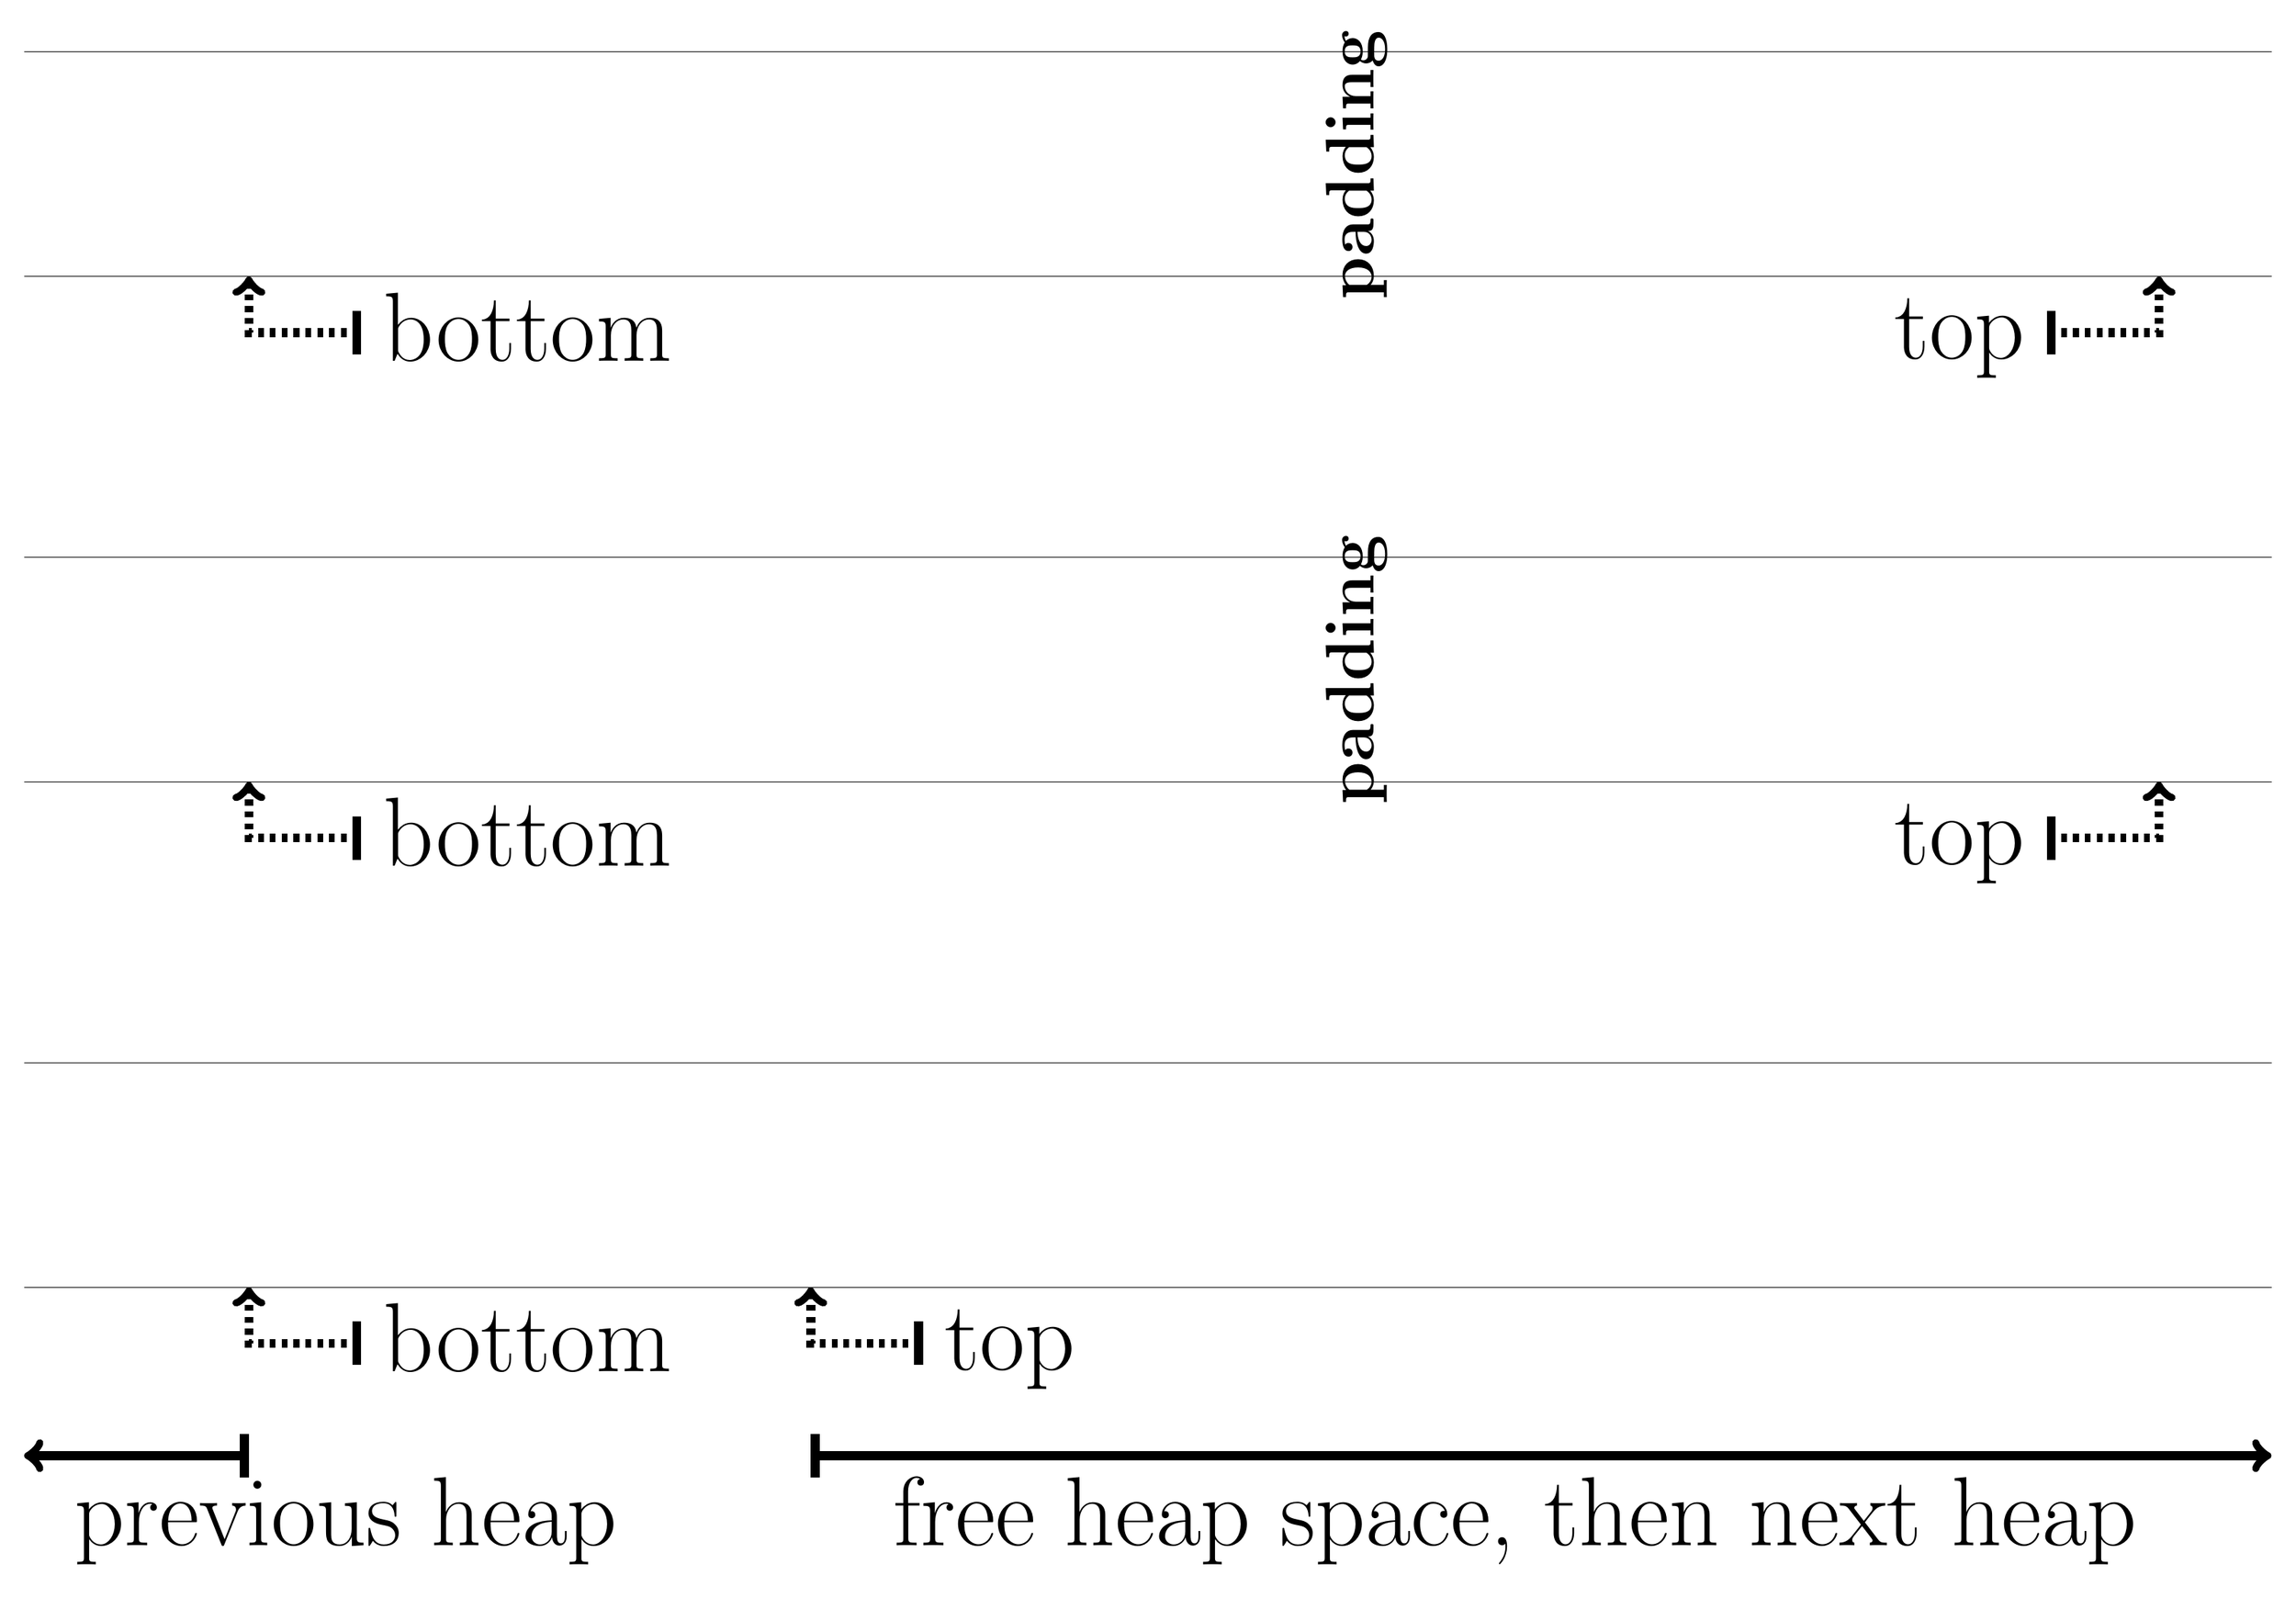
\begin{tikzpicture}[node distance=10mm]

\draw[] (0, 4) -- (40, 4);
\draw[] (0, 0) -- (40, 0);
\WAEntry{4}{14}{col1!30}{postaction={pattern color=gray, pattern=crosshatch}}
\WAEntry{14}{23}{col2!30}{postaction={pattern color=gray, pattern=crosshatch}}
\WAEntry{24}{38}{col3!30}{postaction={pattern color=gray, pattern=crosshatch}}
\WALink{14}{24}{1}
\WALink{4}{14}{0}
\WALinkFwd{24}{38}{0}
\node[scale=1.4,anchor=north, rotate=90] at (23, 2) {\Huge\textbf{padding}};
\draw[line width=4.5, <-|,dashed] (4, 0) -- (4, -1) -- (6, -1) node[scale=2.0, anchor=west, yshift=1.5pt] {\Huge{bottom}};
\draw[line width=4.5, <-|,dashed] (38, 0) -- (38, -1) -- (36, -1) node[scale=2.0, anchor=east, yshift=-1.5pt] {\Huge{top}};

\tikzset{shift={(0,-9)}}

\draw[] (0, 4) -- (40, 4);
\draw[] (0, 0) -- (40, 0);
\WAEntry{4}{14}{col1!30}{postaction={pattern color=gray, pattern=crosshatch}}
\WAEntry{14}{23}{col2!30}{}
\WAEntry{24}{38}{col3!30}{postaction={pattern color=gray, pattern=crosshatch}}
\WALink{14}{24}{1}
\WALink{4}{14}{0}
\WALinkFwd{24}{38}{0}
\node[scale=1.4,anchor=north, rotate=90] at (23, 2) {\Huge\textbf{padding}};
\draw[line width=4.5, <-|,dashed] (4, 0) -- (4, -1) -- (6, -1) node[scale=2.0, anchor=west, yshift=1.5pt] {\Huge{bottom}};
\draw[line width=4.5, <-|,dashed] (38, 0) -- (38, -1) -- (36, -1) node[scale=2.0, anchor=east, yshift=-1.5pt] {\Huge{top}};

\tikzset{shift={(0,-9)}}

\draw[] (0, 4) -- (40, 4);
\draw[] (0, 0) -- (40, 0);
\WAEntry{4}{14}{col1!30}{postaction={pattern color=gray, pattern=crosshatch}}
\WALinkFwd{4}{14}{0}

\draw[line width=4.5, <-|,dashed] (4, 0) -- (4, -1) -- (6, -1) node[scale=2.0, anchor=west, yshift=1.5pt] {\Huge{bottom}};
\draw[line width=4.5, <-|,dashed] (14, 0) -- (14, -1) -- (16, -1) node[scale=2.0, anchor=west, yshift=-1.5pt] {\Huge{top}};

\tikzset{shift={(0,-3)}}

\draw[line width=4.5, <-|] (0,0) -- (0.5, 0) node[scale=2.0, anchor=north west] {\Huge{previous heap }} -- (4,0);
\draw[line width=4.5, |->] (14, 0) -- (38,0) node[scale=2.0, anchor=north east] {\Huge{free heap space, then next heap}} -- (40,0);

\end{tikzpicture}

}
\vspace{-2mm}
\caption{Visualization of one chunk in the balanced allocator.
Top: Encoding of three user allocated entries all currently in use, as indicated by the missing grid pattern on the user data.
Middle: Situation after the second entry has been deallocated.
The encoding is not changed to speed up deallocation.
Allocation remains fast as long as sufficient heap space is available to add an entry on top.
Bottom: Situation after the former top entry has been deallocated.
As long as the top entry is unused the space is reclaimed, which makes the scheme especially suitable for balanced allocations and deallocations.
}
\Description{
Visualization of one chunk in the balanced allocator.
Top: Encoding of three user allocated entries all currently in use, as indicated by the missing grid pattern on the user data.
Middle: Situation after the second entry has been deallocated.
The encoding is not changed to speed up deallocation.
Allocation remains fast as long as sufficient heap space is available to add an entry on top.
Bottom: Situation after the former top entry has been deallocated.
As long as the top entry is unused the space is reclaimed, which makes the scheme especially suitable for balanced allocations and deallocations.
}
\label{fig:warp_allocator}
\vspace{-2mm}
\end{figure}

% Probably users can do something like in their code:
% int8_t libomptarget_device_heap_allocator = 0/1;
% And we can put a weak symbol in the device runtime.
We provide two types of allocators: a single-thread generic allocator and a ``balanced'' allocator.
The single-thread generic allocator tracks all allocations in two linked lists: an allocation list and a free list.
Each thread can use the entire heap space if necessary, but access to the lists has to be mutually exclusive, which can become a performance bottleneck for applications that allocate heap memory concurrently.
The balanced allocator is designed to mitigate this limitation.
It divides the heap space into $N\times{}M$ chunks, with each thread calculating its chunk based on its thread and team id module $N$ and $M$, respectively. 
We use a lock per chunk to ensure consistency, but different chunks are independent.
Since the heap memory each thread can allocate is relatively small, it is possible to run out of memory in only a specific chunk while others are mostly empty.
As it is common to allocate large heap areas in the serial execution part of a program, the first chunk of the $N$ is larger than the rest (with a configurable ratio).
Since the initial thread is always the first thread of a warp / wavefront, it has consequently more heap available when it executes the sequential program parts.

% In contrast to the single-threaded allocator, the warp allocator does not use explicit linked lists but instead embeds indices/pointers into the allocation metadata.
% The concept is visualized in \Cref{fig:malloc} for a single chunk.
% The top row contains three allocations that are in use, as indicated by the grid pattern over the user data.
% When the middle entry is deallocated, it is marked as such but the now free memory is kept in place and not referenced anywhere else.
% To reuse previously deallocated memory regions that have not been reclaimed we need to walk the list until a suitable entry is found, which is costly in practice.
% Consequently, we avoid reusing allocations until we run out of heap space in this chunk.
% Whenever the top allocation is not used anymore we reclaim it by moving the watermark pointer to the end of the previous entry.
% The newly formed top might be reclaimed as well if it was deallocated before.
% The third row in the figure shows the situation after the top entry was deallocated and the two top entries have been reclaimed.

% Overall, this scheme is not a replacement for a more generic allocator.
% However, it is well suited for applications with balanced allocations and deallocations, in terms of lifetime, since we can reclaim memory with minimal overhead during the allocation and deallocation calls.
% In the worst case, allocations with different lifetime are interleaved which will cause holes and costly linear traversals as soon as the heap space runs out.
% However, if we do not run out of heap space there is likely only minor performance degradation due to the fragmentation.

The balanced allocator differs from the generic allocator in that it embeds indices/pointers into the allocation metadata rather than using explicit linked lists.
\Cref{fig:malloc} illustrates this concept for a single chunk.
The top row displays three allocations that are currently in use, indicated by the grid pattern over the user data.
When the middle entry is deallocated, it is marked as such but the now-free memory is kept in place and not referenced elsewhere.
To reuse previously deallocated memory regions that have not been reclaimed, we need to traverse the list until a suitable entry is found, which can be costly in practice.
Thus, we avoid reusing allocations until we exhaust the heap space in this chunk.
We reclaim the top allocation by moving the watermark pointer to the end of the previous entry whenever the top allocation is no longer in use.
The newly formed top may also be reclaimed if it was previously deallocated.
The third row of the figure illustrates the situation after the top entry was deallocated and the two top entries~have~been~reclaimed.

While this scheme is not a replacement for a more generic allocator, it is well-suited for applications with balanced allocations and deallocations in terms of their lifetime since we can reclaim memory with minimal overhead during the allocation and deallocation calls.
In the worst case, interleaved allocations with different lifetimes cause holes and costly linear traversals as soon as the heap space runs out.
However, if we do not run out of heap space, there is likely only minor performance degradation due to fragmentation.
